% \section{The reciprocal theorem and equaitons for a droplet force and Stresslet}
% \label{ap:reciprocal}




\section{Governing equations and solutions}


At the leading order in droplet volume fraction, the governing equations for $\textbf{u}^*$ and $p_f'$ is equivalent to that of an isolated droplet in an infinite medium \citet{hinch1977averaged}. 
Hence, we consider the problem of an isolated test droplet immersed in an arbitrary flow. 
The disturbances pressure and velocity field relative to the position of a test droplet are noted $\textbf{u}_{o}$, $\textbf{u}_{i}$, $p_{o}$ and $p_{i}$, for the velocity outside the test droplet, the velocity inside the droplet, the pressure outside the droplet and the pressure inside the droplet, respectively. 
In the following the center of mass velocity of the droplet is noted $\textbf{w}$. 
Note that because $\textbf{u}_o$ and $p_o$ are defined as a disturbance fields they vanish far from the position of the test droplets. 
On~\ref{fig:disturbance} we display a schematic representation of the problem. 
\begin{figure}[h!]
    \centering
    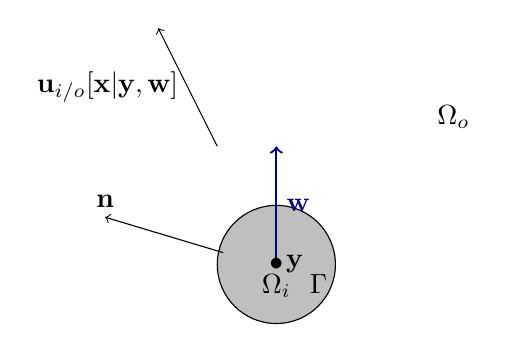
\begin{tikzpicture}[scale= 1.5]
        \filldraw[ gray!50!white](0,0)circle (0.5);
        \draw(0,0)circle (0.5)node[right,below]{   $\;\;\;\;\;\;\;\;\;\;\;\Gamma$};
        \draw[->,blue!50!black,thick](0,0)--++(0,1)node[midway,right]{$\textbf{w}$};
        \draw (0,0)node{$\bullet$}node[right]{$\textbf{y}$};
        \draw[->] (-0.45,0.1)--++(-1,0.3)node[above]{$\textbf{n}$};
        \draw[->](-0.5,1)--++(-0.5,1)node[midway,left]{$\textbf{u}_{i/o}[\textbf{x}|\textbf{y},\textbf{w}]$};
        % \draw[->] (3,1)node{$\bullet$}--++(0,1.5)node[right,midway]{$\textbf{u}_f[\textbf{x}]$};
        \draw (0,0)node[below]{$\Omega_i$};
        \draw (1.5,1.25)node{$\Omega_o$};
    \end{tikzpicture} 
    \caption{Representation of the problem parameters. $\textbf{u}_{o/i}[\textbf{x}|\textbf{y},\textbf{w}]$ is the disturbance velocity field evaluated at \textbf{x}, generated by a test droplet positioned at \textbf{y} with center of mass velocity \textbf{w}. \textbf{n} is the unit normal  pointing outward the droplet. 
    The domain of the exterior of the droplet is noted $\Omega_o$ and the one the interior $\Omega_i$.}
    \label{fig:disturbance}
\end{figure}

\subsection{Maxey, Riley \& Gatignol's equations}

Outside and inside the volume of the test droplet we can write the mass and momentum equations for the disturbances fields, that we note $p_{o/i}$ and $\textbf{u}_{o/i}$, for consitness, by conditionally averaging the Navier stokes equations \citet{koch1993hydrodynamic,fintzi2025}, or simplify by considering the equations derived by \cite{maxey1983equation} \& \citet{gatignol1983faxen}. 
It reads, 
\begin{align}
    \div \textbf{u}_{o} &= 0
    \\
    \div\bm\sigma_{o}
    &= 
    Re [
    \pddt \textbf{u}_{o}
    + \textbf{u}_{o}\cdot \grad \textbf{u}_{o}
    + \textbf{u}_{o}\cdot \grad \textbf{u}_r
    + \textbf{u}_r \cdot \grad \textbf{u}_{o}]
    = Re \textbf{f}_{o}
    \label{eq:momentum_out}
\end{align}
and, 
\begin{align}
    \div \textbf{u}_{i} &= 0,
    \\
    \div\bm\sigma_{i}
    &= 
    \frac{\zeta}{\lambda}Re [
    \pddt \textbf{u}_{i}
    + \textbf{u}_{i}\cdot \grad \textbf{u}_{i}
    + \textbf{u}_{i}\cdot \grad \textbf{u}_r 
    + \textbf{u}_r \cdot \grad \textbf{u}_{i}]
    = \frac{\zeta}{\lambda}Re \textbf{f}_{i}
    \label{eq:momentum_in}
\end{align}
\tb{introduce the dimensionless number (but $\textbf{u}_r$ is acctually unit vect herre) maybe use \textbf{e} it will be clearer for the following}
where we introduced the relative velocity $\textbf{u}_r = \textbf{u} - \textbf{w}$.  
We recall here that \textbf{u} is the undisturbed, or ensemble averaged velocity, present in~\ref{eq:dt_uf2}.
Additionally, $\bm\sigma_{i/o} = -p_{i/o}\bm\delta + 2\textbf{e}_{i/o}$ with $\textbf{e}_{i/o} = \frac{1}{2}[\grad \textbf{u}_{i/o} + ^{\dagger}\grad \textbf{u}_{i/o}]$ is the dimensionless newtonian stresses of each phase. 
% We introduce the Reynolds number $Re = \frac{\rho_f a |\textbf{u}_r|}{\mu_f}$ based on the droplet radius $a$, the density ratio $\zeta = \rho_d / \rho_f$ and the viscosity ratio $\lambda = \mu_d / \mu_f$. 
Note that the distances have been made dimensionless using $a$, and the velocities by $|\textbf{u}_r|$ in the above equation. 

In all rigor, a supplementary term should appear on the right hand side of~\ref{eq:momentum_in,eq:momentum_out}.
This term corresponds to the velocity varience of local velocity field with respect to the conditionally averaged velocity field (see \citet[Chapter 4]{fintzi2025} or \citet{koch1993hydrodynamic}). 
Nevertheless, it has been shown in \citep[Appendix A]{koch1993hydrodynamic} that such contribution is vanishingly small at $O(Re)$ and in the dilute regime. 

At the surface of the droplet ($r = 1$) the continuity of velocity and the non-deformability of the test droplet imposes, 
\begin{align}
    \textbf{u}_{i} = \textbf{u}_{o}
    && 
    \textbf{u}_{i} \cdot \textbf{n}
    =
    - \textbf{u}_r \cdot \textbf{n}
    \label{eq:normal_vel}
\end{align}
where it must be noted that both $\textbf{u}_{i}$ and $\textbf{u}$ are evaluated at the points on the surface of the droplet, hence $\textbf{u}_r$ may not always be a constant vector. 
The undisturbed or ensemble averaged shear rate of the continuous phase reads  $\textbf{E} =\frac{1}{2} [\grad \textbf{u} + ^\dagger \grad \textbf{u}]$. 
Note that for instance the ensemble averaged quantities $\textbf{u}$ and $\textbf{E}$ are kept general, hence their values depends on the position along the surface of the test droplet. 
At the interface of the test droplet the tangential shear rate is assumed continuous, however because it is the total shear rate field (and not just $\textbf{e}_{i/o}$) that satisfy this condition, we obtain (at $r=1$),
\begin{equation}
    \mathbf{n}\cdot [\textbf{e}_{o} - \lambda \textbf{e}_{i} + (1-\lambda)\textbf{E}
    % - \textbf{b}
    ]\cdot (\bm\delta - \textbf{nn})
    =
    \textbf{b}\cdot (\bm\delta - \textbf{nn})
    % 0
    \label{eq:boundary_cdt_stress}
\end{equation}
with, 
\begin{equation}
    \textbf{b}
    =
    \frac{a \grad \gamma}{2 \mu_f |\textbf{u}_r|}
    = Ma \grad\gamma /|\grad \gamma|. 
\end{equation}
Where we have considered Marangoni stresses, with $Ma = \frac{a |\grad \gamma|}{2 \mu_f |\textbf{u}_r|}$. 



% where we have introduced the relative velocity field $\textbf{U}[\textbf{x},t] = \textbf{w} - \textbf{U}_f[\textbf{x},t]$. 
Far from the test droplet it is assumed that the disturbance fields are small, hence the final requirement on $p_{o}$ and $\textbf{u}_{o}$ are, 
\begin{align*}
    \lim_{|\textbf{x}-\textbf{y}|\to\infty }\textbf{u}_{o}[\textbf{x}|\textbf{y},\textbf{w}] = 0,
    && \lim_{|\textbf{x}-\textbf{y}|\to\infty }p_{o}[\textbf{x}|\textbf{y},\textbf{w}]= 0. 
\end{align*}
We recall that $\textbf{y}$ is the position of the test droplet and \textbf{x} a point of evaluation. 





\subsection{Stokes flow solution for a droplet embedded in a quadratic flow}
The Reciprocal theorem requires the use of a known solution.
We call that solution the \textit{test} solution, since its only purpose is to compute the \textit{real} solution of the equations introduced above. 
We note the \textit{test} velocity and stress fields $\hat{\textbf{u}}_{i/o}$ and $\hat{\bm\sigma}_{i/o} = - \hat{p}_{i/o}\bm\delta + \grad \hat{\textbf{u}}_{i/o} + ^\dagger\grad \hat{\textbf{u}}_{i/o}$, respectively. 

In this problem we neglect all inertial effects and consider an arbitrary quadratic flow. 
In this situation $\hat{p}_{out/in}$ and $\hat{\textbf{u}}_{out/in}$ satisfy,
\begin{align}
    \div \hat{\textbf{u}}_{o} = 0 
    &&\div\hat{\bm\sigma}_{o}  = 0 
    \label{eq:momentum_out_s}\\
    \div \hat{\textbf{u}}_{i} = 0 
    && \div\hat{\bm\sigma}_{i}  = 0 
    \label{eq:momentum_in_s}
\end{align}
with the boundary conditions, 
\begin{equation}
    \lim_{|\textbf{x}-\textbf{y}|\to \infty}(\hat{\textbf{u}}_{o},p_{o}) = (\textbf{0},0) 
\end{equation}
and (at $r=1$),
\begin{align}
    \hat{\textbf{u}}_{i} &= \hat{\textbf{u}}_{o}\\
    \hat{\textbf{u}}_{i} \cdot \textbf{n} &= - \hat{\textbf{u}}_r \cdot \textbf{n}
    \label{eq:normal_vel_s}
    \\
    \mathbf{n}\cdot [\hat{\textbf{e}}_{o} - \lambda \hat{\textbf{e}}_{i} + (1-\lambda) \hat{\textbf{E}}
    % - \hat{\textbf{b}}
    ]\cdot (\bm\delta - \textbf{nn})
    &=
    \hat{\textbf{b}}\cdot (\bm\delta - \textbf{nn})
    % 0
\end{align}
where we introduced $\hat{\textbf{u}}_r = \hat{\textbf{u}} - \textbf{w}$ as the ensemble or undisturbed velocity field of the test problem, similarly $\hat{\textbf{E}}$ is the undisturbed stress of the test problem. 


For our purposes we only need $\hat{\textbf{b}}$ and $\hat{\textbf{u}}$ to be quadratic fields.
Hence, we introduce the relations, 
\begin{align*}
    \hat{\textbf{u}}(\textbf{y} + \textbf{n}) 
    &=  \hat{\textbf{u}}_r|_{\textbf{r}=0}
    +  \textbf{r} \cdot  \grad\hat{\textbf{u}}|_{\textbf{r}=0}
    +  \frac{1}{2}\textbf{rr} :  \grad\grad\hat{\textbf{u}}|_{\textbf{r}=0}
    + \ldots\\
     \hat{\textbf{E}}(\textbf{y} + \textbf{n}) 
    &=   \hat{\textbf{E}}|_{\textbf{r}=0}
    + \textbf{r} \cdot  \grad \hat{\textbf{E}}|_{\textbf{r}=0}
    + \frac{1}{2}\textbf{rr} :  \grad\grad \hat{\textbf{E}}|_{\textbf{r}=0}
    + \ldots\\
     \hat{\textbf{b}}(\textbf{y} + \textbf{n}) 
    &=   \hat{\textbf{b}}|_{\textbf{r}=0}
    + \textbf{r} \cdot  \grad \hat{\textbf{b}}|_{\textbf{r}=0}
    + \frac{1}{2}\textbf{rr} :  \grad\grad \hat{\textbf{b}}|_{\textbf{r}=0}
    + \ldots
\end{align*}
\tb{note that we don't consider the symmetry between gradient hence $\grad\grad\hat{\textbf{u}}\approx $ arbitrary tensor; this is already what is considered }
According to the linearity of the Stokes equations we deduce that $\textbf{u}_{i/o}$ and $p_{i/o}$  must be linear combination of spherical harmonics proportional to $\textbf{u}|_{\textbf{x}=0}$, $\grad \gamma|_{\textbf{x}=0}$, and their derivatives \citep{brenner1963resistance}.
Hence, we can write that the disturbance velocity and pressure fields are given by, 
\begin{align}
    \begin{pmatrix}
        \hat{\textbf{u}}_{o}\\
        \hat{p}_{o}\\
        \hat{\textbf{u}}_{i}\\
        \hat{p}_{i}
    \end{pmatrix}
    =
    \begin{pmatrix}
        \textbf{U}_{o}^{(1)} + \textbf{U}_{o}^{(2)}\cdot \grad + \textbf{U}_{o}^{(3)} :\grad\grad &
        \textbf{U}_{o}^\text{(b-1)} + \textbf{U}_{o}^\text{(b-2)}\cdot \grad + \textbf{U}_{o}^\text{(b-3)} :\grad\grad \\
        \textbf{P}_{o}^{(1)} + \textbf{P}_{o}^{(2)}\cdot \grad + \textbf{P}_{o}^{(3)} :\grad\grad &
        \textbf{P}_{o}^\text{(b-1)} + \textbf{P}_{o}^\text{(b-2)}\cdot \grad + \textbf{P}_{o}^\text{(b-3)} :\grad\grad \\
        \textbf{U}_{i}^{(1)} + \textbf{U}_{i}^{(2)}\cdot \grad + \textbf{U}_{i}^{(3)} :\grad\grad &
        \textbf{U}_{i}^\text{(b-1)} + \textbf{U}_{i}^\text{(b-2)}\cdot \grad + \textbf{U}_{i}^\text{(b-3)} :\grad\grad \\
        \textbf{P}_{i}^{(1)} + \textbf{P}_{i}^{(2)}\cdot \grad + \textbf{P}_{i}^{(3)} :\grad\grad &
        \textbf{P}_{i}^\text{(b-1)} + \textbf{P}_{i}^\text{(b-2)}\cdot \grad + \textbf{P}_{i}^\text{(b-3)} :\grad\grad \\
    \end{pmatrix}
    \cdot 
    \begin{pmatrix}
        \hat{\textbf{u}}_r\\
        \hat{\textbf{b}}
    \end{pmatrix}
    \label{eq:big_solution}
\end{align}
The tensor $\textbf{U}_{i/o}^{(n)}$ and $\textbf{P}_{i/o}^{(n)}$ are $n+1$ and $n$ order tensors given in \citet[Appendix F]{fintzi2024averaged}, that depend only on the coordinate $\textbf{r} = \textbf{x}-\textbf{y}$ and the viscosity ratio $\lambda$.
We also define the $n+2$ order tensors\footnote{The $^\dagger$ is used to indicate the transpose operator which acts on the two closet index, example the triadic $^\dagger\textbf{abc} = \textbf{bac}$ while $\textbf{abc}^\dagger = \textbf{acb}$. }, 
\begin{equation}
    \textbf{S}_{i/o}^{(n)} = 
    - \bm\delta\textbf{P}_{i/o}^{(n)}
    + \grad \textbf{U}_{i/o}^{(n)}
    + ^\dagger\grad \textbf{U}_{i/o}^{(n)},
    \label{eq:big_S}
\end{equation}
which provide the stresses fields upon contraction with $\textbf{u}_r$, $\textbf{b}$, and the higher derivatives. 

\subsection{Point source solution}



Following \citet{stone2001inertial} we also consider the test problem of a point source located at the origin.
In this case the test velocity  and stress fields, follow the equations, $\div\bm\sigma_{i/o}=\grad \delta(\textbf{r})$ and $\div \textbf{u}_{i/o}$, and the solutions read \citep{pozrikidis2011introduction,pozrikidis1992boundary} (see also~\ref{ap:second_mom}), 
\begin{align}
    \hat{\textbf{u}}_{o/i} = \frac{Q}{4\pi} \textbf{n}r^{-2}
    && \hat{\bm\sigma}_{o/i} = \mu_f \frac{Q}{2\pi}\left(
        \bm\delta
        - 3 \textbf{nn}
    \right)r^{-3}
    \label{eq:point_source}
\end{align}
Note that this expression is valid throughout the domain excluding the point $\textbf{r} =  \textbf{x} -  \textbf{y} = 0$, hence we may use either the subscript $o$ or $i$. 
The reason why this solution is necessary is because, in the previous test problem $\div \hat{\textbf{u}}= 0$ (in opposition to what we have in~\ref{eq:point_source} where $\div \textbf{u} = Q \delta(\textbf{x})$), hence the previous solution was unable to provide a formula for the trace of the first moment using the reciprocal theorem \citep{stone2001inertial}.

In summary, as the values of $\hat{\textbf{u}}_r$, $\hat{\textbf{b}}$ and $Q$ are entirely arbitrary, the solutions given by~\ref{eq:big_solution} and~\ref{eq:point_source} will be used as a tool to derive formula for the drag forces, first moment, and second moment of hydrodynamic forces, using the reciprocal theorem derived in the next section.  

\section{Reciprocal theorem for droplets}

% We now demonstrate how to derive the reciprocal theorem for droplets.
A similar derivation to what is presented here may be found in \citet{lovalenti1993force,raja2010inertial}, however we hope to provide some clarifications and generalization, by exposing a detailed and simpler demonstration.  

The derivation of the general formula goes into three steps: (1) we write the reciprocal theorem in the exterior of the droplet, (2) then on the interior of the droplet, (3) then using the boundary condition at the interface of the droplet we write the final formula. 

\subsection{First step:}
We first take the dot product of~\ref{eq:momentum_out} with $\hat{\textbf{u}}_{o}$, and the dot product of~\ref{eq:momentum_out_s} with $\textbf{u}_{o}$, subtracting both expression gives, 
\begin{equation}
    \div (\bm\sigma_{o}\cdot \hat{\textbf{u}}_o)
    % - \bm\sigma_o :\grad \hat{\textbf{u}}_o
    % \hat{\textbf{u}}_{o} \cdot (\div \bm\sigma_{o})
    =
    \div (\hat{\bm\sigma}_{o}\cdot \textbf{u}_o)
    % - \hat{\bm\sigma}_o :\grad \textbf{u}_o
    + Re (\hat{\textbf{u}}_{o}\cdot \textbf{f}_{o}). 
    \label{eq:first_step_out}
\end{equation}
To derive this relation we used the fact that $\bm\sigma_o :\grad \hat{\textbf{u}}_o = 2\textbf{e}_o :\grad \hat{\textbf{u}}_o = 2{\textbf e}_o : \hat{\textbf e}_o$, and  $\hat{\bm\sigma}_o :\grad {\textbf{u}}_o = 2\hat{\textbf{e}}_o : \textbf{e}_o$, leading to $\bm\sigma_o :\grad \hat{\textbf{u}}_o = \hat{\bm\sigma}_o :\grad {\textbf{u}}_o$. 
This simplification is the reason why the complete knowledge of the velocity field becomes unnecessary with the reciprocal theorem when $\textbf{f}_o = 0$.
Consequently, the  efficiency of the reciprocal theorem is rooted in the commutativity of the operation $\textbf e_o:\hat{\textbf e}_o$. 
Integrating this expression on the whole domain $\Omega_{o}$, and injecting the relations $\textbf{u}_o = \textbf{u}_o+\textbf{u}_r-\textbf{u}_r$ and $\hat{\textbf{u}}_o = \hat{\textbf{u}}_o+\hat{\textbf{u}}_r-\hat{\textbf{u}}_r$ gives, 
\begin{equation}
    \intS[p]{\hat{\textbf{u}}_{r} \cdot  \bm\sigma_{o}\cdot \textbf{n}}
    - 2\intS[p]{(\hat{\textbf{u}}_{o} + \hat{\textbf{u}}_r) \cdot  \textbf e_{o}\cdot \textbf{n}}
    =
    \intS[p]{\textbf{u}_{r}\cdot \hat{\bm\sigma}_{o}\cdot \textbf{n}}
    - 2\intS[p]{(\textbf{u}_{o} + \textbf{u}_r)\cdot \hat{\textbf e}_{o}\cdot \textbf{n}}
    + 
    Re\intO[o]{\hat{\textbf{u}}_{o}\cdot \textbf{f}_{o}}.
    \label{eq:int_first_step}
\end{equation}
Where we used the relation, $(\hat{\textbf{u}}_{o} + \hat{\textbf{u}}_r) \cdot  \bm\sigma_{o}\cdot \textbf{n} = 2 (\hat{\textbf{u}}_{o} + \hat{\textbf{u}}_r) \cdot  \textbf e_{o}\cdot \textbf{n}$, allowed  because $(\hat{\textbf{u}}_{o} + \hat{\textbf{u}}_r) = (\bm\delta - \textbf{nn})\cdot (\hat{\textbf{u}}_{o} + \hat{\textbf{u}}_r)$ on the surface of the test droplet, see~\ref{eq:normal_vel_s}. 
Similar considerations lead to $({\textbf{u}}_{o} + {\textbf{u}_r}) \cdot  \hat{\bm\sigma}_{o}\cdot \textbf{n} =2  ({\textbf{u}}_{o} + {\textbf{u}_r}) \cdot  \hat{\textbf e}_{o}\cdot \textbf{n}$. 
\ref{eq:int_first_step} is the correct expression of the reciprocal theorem if one consider solid particles.
Indeed, in that case $\hat{\textbf{u}}_{o}$ is imposed by the no-slip boundary condition at the particle interface, hence leading directly to a formula for the force traction on the surface of the solid particle (first term on the left-hand side of~\ref{eq:int_first_step}). 
For fluid particles few more steps are necessary. 

\subsection{Second step:}

We now take the dot product of~\ref{eq:momentum_in} with $(\hat{\textbf{u}}_i + \hat{\textbf{u}}_r)$ and of~\ref{eq:momentum_in_s} with $(\textbf{u}_i+ \textbf{u}_r)$, subtracting both expression leads to, 
\begin{equation}
    \div [\bm\sigma_{i}\cdot (\hat{\textbf{u}}_i+\hat{\textbf{u}}_r)]
    - 2\textbf{e}_i : \hat{\textbf{E}}
    % \hat{\textbf{u}}_{i} \cdot (\div \bm\sigma_{i})
    =
    \div [\hat{\bm\sigma}_{i}\cdot (\textbf{u}_i+\textbf{u}_r)]
    - 2\hat{\textbf{e}}_i :\textbf{E}
    + \frac{\zeta}{\lambda} Re (\hat{\textbf{u}}_i+\hat{\textbf{u}}_r)\cdot \textbf{f}_{i}. 
    \label{eq:second_step_out}
\end{equation}
where we used the relation, $- \bm\sigma_i :\grad (\hat{\textbf{u}}_i+\hat{\textbf{u}}_r)+ \hat{\bm\sigma}_i :\grad ({\textbf{u}}_i+{\textbf{u}}_r) =
- 2\textbf{e}_i :\hat{\textbf{E}} + 2\hat{\textbf{e}}_i :\textbf{E}$. 
% We recall that $\hat{\bm\tau}_f$ and $\bm\tau_f$ correspond to the ensemble averaged stress fields of the test problem and true problem, respectively. 
Integrating this relation over the domain $\Omega_i$, and using the divergence theorem, as well as similar simplifications used in~\ref{eq:int_first_step}, gives, 
\begin{equation}
    \intS[p]{ (\hat{\textbf{u}}_i+\hat{\textbf{u}}_r)\cdot \textbf{e}_{i}\cdot\textbf{n}}
    - \intO[i]{\textbf{e}_i : \hat{\textbf{E}}}
    =
    \intS[p]{ (\textbf{u}_i+\textbf{u}_r)\cdot\hat{\textbf{e}}_{i}\cdot \textbf{n}}
    - \intO[i]{\hat{\textbf{e}}_i :\textbf{E}}
    + \frac{\zeta}{2\lambda} Re \intO{(\hat{\textbf{u}}_i+\hat{\textbf{u}}_r)\cdot \textbf{f}_{i}} 
    \label{eq:second_step_int}
\end{equation}
Because $(\hat{\textbf{u}}_i+\hat{\textbf{u}}_r)\cdot (\bm\delta-\textbf{nn}) = (\hat{\textbf{u}}_i+\hat{\textbf{u}}_r)$, multiplying~\ref{eq:boundary_cdt_stress} by $(\hat{\textbf{u}}_i+\hat{\textbf{u}}_r)$ gives the appropriate boundary condition for the first integral on the left-hand side of~\ref{eq:second_step_int}, namely,
\begin{equation}
    \mathbf{n}\cdot [
        \textbf{e}_{o} - \lambda \textbf{e}_i 
        + (1 -\lambda) \textbf{E}
        % - \textbf{b}
        ]\cdot (\hat{\textbf{u}}_{i/o}+\hat{\textbf{u}}_r)
        =
        \textbf{b}\cdot (\hat{\textbf{u}}_{i/o}+\hat{\textbf{u}}_r)
    \label{eq:boundary_with_the_velocity}
\end{equation}
with a similar relation for the test problem boundary condition and $({\textbf{u}}_{i/o}+{\textbf{u}}_r)$ in the first integral on the right-hand side of~\ref{eq:second_step_int}. 

Adding~\ref{eq:int_first_step} and~\ref{eq:second_step_int} times $\lambda$, while using the boundary condition given by~\ref{eq:boundary_with_the_velocity} leads to the expression,
\begin{multline}
    \intS[p]{\hat{\textbf{u}}_{r} \cdot  \bm\sigma_{o}\cdot \textbf{n}}
    -\lambda \intO[i]{2\textbf{e}_i : \hat{\textbf{E}}}
    - (1-\lambda) \intS[p]{2(\textbf{u}_{i} + \textbf{u}_r)\cdot \hat{\textbf{E}}\cdot \textbf{n}}
    + \intS[p]{2(\textbf{u}_{i} + \textbf{u}_r)\cdot \hat{\textbf{b}}}
    \\
    =
    \intS[p]{\textbf{u}_{r}\cdot \hat{\bm\sigma}_{o}\cdot \textbf{n}}
    - \lambda \intO[i]{2\hat{\textbf{e}}_i :\textbf{E}}
    - (1-\lambda) \intS[p]{2(\hat{\textbf{u}}_{i} + \hat{\textbf{u}}_r) \cdot  \textbf{E} \cdot \textbf{n}}\\ 
    + \intS[p]{2(\hat{\textbf{u}}_{i} + \hat{\textbf{u}}_r) \cdot  \textbf{b}}
    + \zeta Re \intO{(\hat{\textbf{u}}_i+\hat{\textbf{u}}_r)\cdot \textbf{f}_{i}} 
    + Re\intO[o]{\hat{\textbf{u}}_{o}\cdot \textbf{f}_{o}}.
    \label{eq:int_third_step}
\end{multline}

\subsection{Final step:}

To obtain the ``final form'' of the reciprocal theorem we proceed by noting that the second and third terms on the left-hand side  of~\ref{eq:int_third_step} may be combined upon using the divergence theorem on the third term, and using the relation, 
\begin{equation}
    - \lambda \textbf{e}_i : \hat{\textbf{E}}
    - (1-\lambda)\div [\hat{\textbf{E}} \cdot (\textbf{u}_i + \textbf{u}_r)]
    =
    % - \lambda \textbf{e}_i : \hat{\textbf{E}}
    % - (1-\lambda) \hat{\textbf{E}}:(\textbf{e}_i + \textbf{E})
    - \textbf{e}_i : \hat{\textbf{E}}
    - (1-\lambda) \hat{\textbf{E}}:\textbf{E}
    - (1-\lambda)\div \hat{\textbf{E}} \cdot (\textbf{u}_i + \textbf{u}_r).
    \label{eq:tricks_two}
\end{equation}
One can also derive the same manipulation on the second and third term on the right-hand side of~\ref{eq:int_third_step}, namely,
\begin{equation}
    - \lambda \hat{\textbf{e}}_i : {\textbf{E}}
    - (1-\lambda)\div [{\textbf{E}} \cdot (\hat{\textbf{u}}_i + \hat{\textbf{u}}_r)]
    =
    % - \lambda \textbf{e}_i : \hat{\textbf{E}}
    % - (1-\lambda) \hat{\textbf{E}}:(\textbf{e}_i + \textbf{E})
    - \hat{\textbf{e}_i} : {\textbf{E}}
    - (1-\lambda) \hat{\textbf{E}}:\textbf{E}
    - (1-\lambda)\div {\textbf{E}} \cdot (\hat{\textbf{u}}_i + \hat{\textbf{u}}_r)
    \label{eq:tricks_one}
\end{equation}
Because the product $\hat{\textbf{E}} : {\textbf{E}}$ is commutative, the second term on the right-hand side of~\ref{eq:tricks_one} and~\ref{eq:tricks_two} cancel each other in the final expression.  
Injecting both~\ref{eq:tricks_one} and~\ref{eq:tricks_two} in~\ref{eq:int_third_step} leads to the final form of the reciprocal theorem for droplets, 
\begin{multline}
    \intS[p]{\hat{\textbf{u}}_{r} \cdot  \bm\sigma_{o}\cdot \textbf{n}}
    - \intO[i]{2\textbf{e}_i : \grad\hat{\textbf{u}}}
    - (1-\lambda) \intO[p]{(\textbf{u}_{i} + \textbf{u}_r)\cdot \grad^2 \hat{\textbf{u}}}
    + \intS[p]{2(\textbf{u}_{i} + \textbf{u}_r)\cdot \hat{\textbf{b}}}
    \\
    =
    \intS[p]{\textbf{u}_{r}\cdot \hat{\bm\sigma}_{o}\cdot \textbf{n}}
    - \intO[i]{2\hat{\textbf{e}}_i :\grad\textbf{u}}
    - (1-\lambda) \intO[p]{(\hat{\textbf{u}}_{i} + \hat{\textbf{u}}_r) \cdot \grad^2 \textbf{u} }\\ 
    + \intS[p]{2(\hat{\textbf{u}}_{i} + \hat{\textbf{u}}_r) \cdot  \textbf{b}}
    + \zeta Re \intO{(\hat{\textbf{u}}_i+\hat{\textbf{u}}_r)\cdot \textbf{f}_{i}} 
    + Re\intO[o]{\hat{\textbf{u}}_{o}\cdot \textbf{f}_{o}}.
    \label{eq:int_final_step}
\end{multline}
Note that we used the relations, $2{\textbf{e}_i} : \hat{\textbf{E}} = 2{\textbf{e}_i} : {\grad\textbf{u}}$ and $\div\textbf{E} = \frac{1}{2}\grad^2 \textbf{u}$ because the background flow is divergence free. 
Upon making the good choice for $(\hat{\textbf{E}}, \hat{\textbf{u}}_r)$, one recover on the left-hand side of~\ref{eq:int_final_step} the expression of the drag force and the first, second and higher moments in present in~\ref{eq:f_alpha} and~\ref{eq:def_sigma_eff_f}, respectively. 
The note that on the right-hand side of~\ref{eq:int_final_step} all the terms, are either, known quantities from the ``test'' problem ($\hat{\bm\sigma}_{o},\hat{\textbf{e}}_i, \hat{\textbf{u}}_{i/o/r}$), or far-field condition of the ``real'' problem ($\textbf{E},\textbf{u}_r$). 
However, one exception remain, that is the inertial term $\textbf{f}_{i/o}$ to be evaluated in the whole domain $\Omega$, which is a function of the unknown velocity field $\textbf{u}_{i/o}$. 

Hence, to compute the right-hand-side~\ref{eq:int_final_step} one must proceed by applying some approximation allowing us to obtain the last two terms of~\ref{eq:int_final_step}. 
This is the subject of the next section. 




\section{Moments of force on a translating droplet}

In this section we provide the general formulation to derive the drag force, first moments of forces, and second moment of forces, i.e. for~\ref{eq:f_alpha}, and second, and third term of~\ref{eq:def_sigma_eff_f}, respectively. 
Likewise, we demonstrate how to obtain a formula for the droplet internal shear integrated over its volume, and the first moment of the droplet internal shear.
These two quantities are useful to determine the droplet deformation.  

Once these formulas are properly stated, we consider the case of a droplet embedded in a uniform flow (i.e. when $\textbf{u}_r$ is a uniform vector field), and small but finite Reynolds number. 
In this context we derive a new formula for the first moment of the forces (i.e. for the Stresslet tensor), and conclude on what are the implication on the Rheology of the mixture given by~\ref{eq:def_sigma_eff_f}. 


\subsection{General formula for the force, first and second moments}
Let us consider four configurations for the test problem, namely,
\begin{center}
    \begin{tabular}{|cccc|}\hline
        Configurations & $\hat{\textbf{u}}_r(\textbf{x})$&$\hat{\textbf{b}}(\textbf{x})$ & $Q(\textbf{x})$\\ \hline
        1 & $\hat{\textbf{u}}_r = \hat{\textbf{u}}_r(\textbf{y})$& $\hat{\textbf{b}} = 0$ & $Q= 0$\\
        2 & $\hat{\textbf{u}}_r = \textbf{r}\cdot \grad \hat{\textbf{u}}$& $\hat{\textbf{b}} = 0$ & $Q= 0$\\
        3 & $\hat{\textbf{u}}_r = 0$& $\hat{\textbf{b}} = 0$ & $Q=Q(\textbf{y}) $\\
        4 & $\hat{\textbf{u}}_r = 0$& $\hat{\textbf{b}} = \textbf{r}\cdot \grad\hat{\textbf{b}}$ & $Q= 0$\\ \hline
    \end{tabular}
\end{center}
whether it is for configuration 1, 2, 3 or 4, one can obtain the expression of $\hat{\bm\sigma}_{i/o}$ and $\hat{\textbf{u}}_{i/o}$ needed in~\ref{eq:int_final_step} from~\ref{eq:big_solution},~\ref{eq:big_S} and~\ref{eq:point_source}. 
% \begin{align}
%     \label{eq:ur_cst}
%     \hat{\textbf{u}}_r = \hat{\textbf{u}}_r|_{\textbf{x}=\textbf{y}} 
%     && 
%     \hat{\textbf{b}} = 0 &&\text{Solutions: } 
%     && 
%     \hat{\textbf{u}}_{o/i} = \textbf{U}_{o/i}^{(1)}\cdot \hat{\textbf{u}}_r|_{\textbf{x}=\textbf{y}} 
%     && 
%     \hat{\bm\sigma}_{o/i} = \textbf{S}_{o/i}^{(1)}\cdot \hat{\textbf{u}}_r|_{\textbf{x}=\textbf{y}}, \\
%     \label{eq:grad_ur_cst}
%     \hat{\textbf{u}}_r =\textbf{r}\cdot  \grad \textbf{u}|_{\textbf{x}=\textbf{y}} 
%     && 
%     \hat{\textbf{b}} = 0 &&\text{Solutions: } 
%     && 
%     \hat{\textbf{u}}_{o/i} = \textbf{U}_{o/i}^{(2)} : \grad\hat{\textbf{u}}|_{\textbf{x}=\textbf{y}} 
%     && 
%     \hat{\bm\sigma}_{o/i} = \textbf{S}_{o/i}^{(2)} : \grad\hat{\textbf{u}}|_{\textbf{x}=\textbf{y}}, 
% \end{align}

Setting configuration $1)$ into~\ref{eq:int_final_step} gives, 
\begin{multline}
    \intS[p]{\bm\sigma_{o}\cdot \textbf{n}}
    % - \intO[i]{2\textbf{e}_i : \grad\hat{\textbf{u}}}
    % - (1-\lambda) \intO[p]{(\textbf{u}_{i} + \textbf{u}_r)\cdot \grad^2 \hat{\textbf{u}}}
    % + \intS[p]{2(\textbf{u}_{i} + \textbf{u}_r)\cdot \hat{\textbf{b}}}
    =
    \intS[p]{\textbf{u}_{r}\cdot \textbf{S}_{o}^{(1)}\cdot \textbf{n}}
    - \intO[i]{ \textbf{S}_{i}^{(1)} :\grad\textbf{u}}
    - (1-\lambda) \intO[p]{(\textbf{U}_{i}^{(1)} + \bm\delta) \cdot \grad^2 \textbf{u} }\\ 
    + \intS[p]{2 (\textbf{U}_{i/o}^{(1)} + \bm\delta) \cdot  \textbf{b}}
    + \zeta Re \intO{(\textbf{U}_{i}^{(1)} + \bm\delta)\cdot \textbf{f}_{i}} 
    + Re\intO[o]{\textbf{U}_{o}^{(1)}\cdot \textbf{f}_{o}},
    \label{eq:drag_force}
\end{multline}
Which is a general formula for the hydrodynamic drag forces. 
Based on this formula, one can re-derive the famous Faxen law, or even the BBO model \citep{kim2013microhydrodynamics}. But in this work we rather focus on the first moment of force. 

The general formula for the first moment of force may be obtained setting configuration 2) into~\ref{eq:int_final_step}, it yields,
\begin{multline}
    \intS[p]{r_j(\bm\sigma_{o}\cdot \textbf{n})_i}
    - \intO[i]{2(\textbf{e}_i)_{ij}}
    % - (1-\lambda) \intO[p]{(\textbf{u}_{i} + \textbf{u}_r)\cdot \grad^2 \hat{\textbf{u}}}
    % + \intS[p]{2(\textbf{u}_{i} + \textbf{u}_r)\cdot \hat{\textbf{b}}}
    % \\
    \overset{i\neq j}{=}
    \intS[p]{(\textbf{u}_{r})_l (\textbf{S}^{(2)}_{o})_{ijkl} n_k}
    - \intO[i]{(\textbf{S}^{(2)}_{i})_{ijkl}(\grad\textbf{u})_{kl}}\\
    - (1-\lambda) \intO[p]{(\textbf{U}_{i}^{(2)} + \textbf{r}\bm\delta)_{ijk} (\grad^2 \textbf{u})_k }
    + \intS[p]{2(\textbf{U}_{i}^{(2)} + \textbf{r}\bm\delta)_{ijk} b_k}\\
    + \zeta Re \intO{(\textbf{U}_{i}^{(2)} + \textbf{r}\bm\delta)_{ijk} (\textbf{f}_{i})_k} 
    + Re\intO[o]{(\textbf{U}_{o}^{(2)})_{ijk}(\textbf{f}_{o})_k},
    \label{eq:first_mom}
\end{multline}
% \begin{multline}
%     \intS[p]{\textbf{r}\bm\sigma_{o}\cdot \textbf{n}}
%     - \intO[i]{2\textbf{e}_i}
%     % - (1-\lambda) \intO[p]{(\textbf{u}_{i} + \textbf{u}_r)\cdot \grad^2 \hat{\textbf{u}}}
%     % + \intS[p]{2(\textbf{u}_{i} + \textbf{u}_r)\cdot \hat{\textbf{b}}}
%     % \\
%     \overset{Dev}{=}
%     \intS[p]{\textbf{u}_{r}\cdot \textbf{S}^{(2)}_{o}\cdot \textbf{n}}
%     - \intO[i]{\textbf{S}^{(2)}_{i}:\grad\textbf{u}}
%     - (1-\lambda) \intO[p]{(\textbf{U}_{i}^{(2)} + \textbf{r}\bm\delta) \cdot \grad^2 \textbf{u} }\\ 
%     + \intS[p]{2(\textbf{U}_{i}^{(2)} + \textbf{r}\bm\delta) \cdot  \textbf{b}}
%     + \zeta Re \intO{(\textbf{U}_{i}^{(2)} + \textbf{r}\bm\delta)\cdot \textbf{f}_{i}} 
%     + Re\intO[o]{\textbf{U}_{o}^{(2)}\cdot \textbf{f}_{o}},
%     \label{eq:first_mom}
% \end{multline}
It is important to note that to derive~\ref{eq:first_mom} we have factorized the equations by the arbitrary tensors $(\grad \hat{\textbf{u}})_{ij}$. 
Because $(\grad \hat{\textbf{u}})_{kk}=\grad\cdot \hat{\textbf{u}} = 0$, the trace of~\ref{eq:first_mom} gives an erroneous expression because we could not have factorized by zero.  
Hence, it is important to understand that only the traceless part of this equation is meaningful. 
This is the meaning of the ``$i\neq j$'' above the equality sign of~\ref{eq:first_mom}. 
Another way to understand this is that~\ref{eq:first_mom} provides,
\begin{equation}
    M_{ij} - \frac{1}{3}\delta_{ij}M_{kk},
\end{equation}
if $M_{ij}$ were the full first moment for all $i$ and $j$. 

Nevertheless, using configuration 3) directly into~\ref{eq:first_step_out} we obtain a formula for the trace of the first moment, it reads, 
% \begin{align}
%     \hat{\textbf{u}}_{o/i} = \frac{Q}{4\pi} \textbf{n}r^{-2}
%     && \hat{\bm\sigma}_{o/i} = \mu_f \frac{Q}{2\pi}\left(
%         \bm\delta
%         - 3 \textbf{nn}
%     \right)r^{-3}
% \end{align}
\begin{equation}
    \intS[p]{\textbf{r} \cdot  \bm\sigma_{o}\cdot \textbf{n}}
    =
    % + \intS[p]{\textbf{u}_{o}\cdot \textbf{n} \frac{Q}{\pi} r^{-3}}
    - 
    Re\intO[o]{\frac{\textbf{r}}{r^{-3}}\cdot \textbf{f}_{o}}. 
    \label{eq:first_mom_Q}
\end{equation}
Note that the first two terms on the right-hand side of~\ref{eq:first_step_out} vanished in~\ref{eq:first_mom_Q} because $\textbf{u}_o\cdot \hat{\bm\sigma}_o d\Gamma \sim \textbf{u}_o \cdot \textbf{n}d\Gamma$ in this case, and because $\textbf{u}_o$ is assumed incompressible \citep{stone2001inertial}. 

Note that because $\bm\sigma_o$ and $\textbf{e}_i$ are local stresses and shear rates, relative to the bulk stress ($\bm\Sigma$), and bulk shear rate ($\textbf{E}$) the left-hand side term of~\ref{eq:drag_force,eq:first_mom,eq:first_mom_Q,eq:second_mom} are exactly the terms defined in~\ref{eq:f_alpha} and~\ref{eq:def_sigma_eff_f}. 

Although these formulas are sufficient to close the momentum equations presented in introduction, one may be interested into the expression of the integral of $\textbf{e}_i$, independently of the integral of  $\textbf{r}\bm\sigma_o\cdot \textbf{n}$, in opposition to~\ref{eq:first_mom} which provide the resultants of these two terms, i.e $\textbf{r}\bm\sigma_o\cdot \textbf{n}d\Gamma -\textbf{e}_i d\Omega $. 
That is where the configuration 4) comes into place. 
\begin{multline}
    % \intS[p]{\hat{\textbf{u}}_{r} \cdot  \bm\sigma_{o}\cdot \textbf{n}}
    % - \intO[i]{2\textbf{e}_i : \grad\hat{\textbf{u}}}
    % - (1-\lambda) \intO[p]{(\textbf{u}_{i} + \textbf{u}_r)\cdot \grad^2 \hat{\textbf{u}}}
    \intS[p]{2(\textbf{u}_{i} + \textbf{u}_r)\textbf{r}}
    =
    \intS[p]{\textbf{u}_{r}\cdot \textbf{S}_{o}^{(b-2)}\cdot \textbf{n}}
    - \intO[i]{\textbf{S}_{o}^{(b-2)} :\grad\textbf{u}}
    - (1-\lambda) \intO[p]{\textbf{U}_{i}^{(b-2)} \cdot \grad^2 \textbf{u} }\\ 
    + \intS[p]{2\textbf{U}_{i}^{(b-2)} \cdot  \textbf{b}}
    + \zeta Re \intO{\textbf{U}_{i}^{(b-2)}\cdot \textbf{f}_{i}} 
    + Re\intO[o]{\textbf{U}_{o}^{(b-2)}\cdot \textbf{f}_{o}}.
    \label{eq:internal_e}
\end{multline}
Upon using the divergence theorem on the left-hand side term one obtain a formula for the integral of the droplet internal gradient of velocity, which symmetric part corresponds to the integral of $\textbf{e}_i$ over the droplet volume. 

To facilitate reading we report the derivation of the second moment of force expression in~\ref{ap:second_mom}. 


\subsection{Uniform relative motion}

This subsection considers only a uniform relative motion such that $\textbf{u}_r$ is constant of space, and without Marangoni stresses such that $\textbf{b}=0$.

\subsubsection{Drag force}

Here, we re-demonstrate how to obtain the $Re$ contribution to the Drag force, which is a known result \citep{proudman1957expansions, stone2001inertial}. 
This permits us to introduce some notations and provide a clearer picture of the derivation for the following discussions. 

Using~\ref{eq:drag_force} we have, 
\begin{equation}
    \intS[p]{\bm\sigma_{o}\cdot \textbf{n}}
    % - \intO[i]{2\textbf{e}_i : \grad\hat{\textbf{u}}}
    % - (1-\lambda) \intO[p]{(\textbf{u}_{i} + \textbf{u}_r)\cdot \grad^2 \hat{\textbf{u}}}
    % + \intS[p]{2(\textbf{u}_{i} + \textbf{u}_r)\cdot \hat{\textbf{b}}}
    =
    \intS[p]{\textbf{u}_{r}\cdot \textbf{S}_{o}^{(1)}\cdot \textbf{n}}
    % - \intO[i]{ \textbf{S}_{i}^{(1)} :\grad\textbf{u}}
    % - (1-\lambda) \intO[p]{(\textbf{U}_{i}^{(1)} + \bm\delta) \cdot \grad^2 \textbf{u} }\\ 
    % + \intS[p]{2 (\textbf{U}_{i/o}^{(1)} + \bm\delta) \cdot  \textbf{b}}
    + \zeta Re \intO{(\textbf{U}_{i}^{(1)} + \bm\delta)\cdot \textbf{f}_{i}} 
    + Re\intO[o]{\textbf{U}_{o}^{(1)}\cdot \textbf{f}_{o}}. 
    \label{eq:drag_force_application}
\end{equation}
The first term on the right-hand side is by definition the Stokes flow contribution, since $\textbf{u}_{r}\cdot \textbf{S}_{o}^{(1)}$ represents the stress field of a translating spherical droplet in stokes flow condition. 
It yields, 
\begin{equation}
    \intS[p]{\textbf{u}_{r}\cdot \textbf{S}_{o}^{(1)}\cdot \textbf{n}}
    = 2 \pi \frac{2+3\lambda}{\lambda+1} \textbf{u}_r
    =\textbf{f},
    \label{eq:stokes_force}
\end{equation}
where we introduced the vector \textbf{f} to represents the dimensionless Stokes drag force. 

The real challenge is to compute the inertial terms on the right-hand side of~\ref{eq:drag_force} which require an expression for the forcing term $\textbf{f}_o$ and $\textbf{f}_i$. 
In a situation where only uniform relative motions are present we deduce from~\ref{eq:momentum_out,eq:momentum_in} that, 
\begin{equation}
    \textbf{f}_{i/o} = 
    % \pddt \textbf{u}_{i/o} +
    (\textbf{u}_{i/o} + \textbf{u}_r)\cdot \grad \textbf{u}_{i/o},
    \label{eq:inertial_term}
\end{equation}
where we recall that $\textbf{u}_{i/o}$ is the yet unknown inertial velocity fields inside and outside the translating droplet. 
It is well known that at $O(1)$ in $Re$, the fields $\textbf{u}_{i/o}$, can be approximated by $\textbf{u}_{i/o} \approx \textbf{U}^{(1)}_{i/o}\cdot \textbf{u}_r$ only at distance $r < O(Re^{-1})$ \citet{proudman1957expansions}. 
Otherwise, for $r > O(Re^{-1})$, one must use the velocity fields generated by a point force in the Ossen equation, also called a ``Ossenlet'' \citep{pozrikidis2011introduction}. 
So with an accuracy of $O(Re)$ in the final expression, one may use the expression, 
\begin{equation}
    \textbf{u}_{o} = 
    \textbf{u}_{inner}
    + \textbf{u}_{outer}
    - \textbf{G}\cdot \textbf{f}
    =
    \textbf{U}^{(1)}\cdot \textbf{u}_r
    + \textbf{U}^{(out)}\cdot \textbf{f}
    - \textbf{G}\cdot \textbf{f}
    \label{eq:order_1_vel}
\end{equation}
where $\textbf{f}= 2\pi \frac{2+3\lambda}{1+\lambda} \textbf{u}_r$ and $\textbf{G}=(\bm\delta+\textbf{nn})r^{-1}/(8\pi)$ is the green function of Stokes flow. 
This solution is uniformly valid up to $r \to\infty$.
The last term on the right-hand side of this equation is used to remove the ``overlap'' between the inner and outer solution \citet{stone2001inertial}. 
Here $\textbf{U}^{(out)}$ is the ``Ossenlet'' given by \citep{pozrikidis2011introduction}, 
\begin{equation}
    \textbf{U}^{(out)}
    = \frac{e^X}{4\pi r}\bm\delta
    + \grad \left(
        \frac{e^X-1}{8\pi}
        (\textbf{u}_r - \textbf{n})
    \right)
\end{equation}
with $X = \frac{Re}{2} r (\textbf{u}_r \cdot \textbf{n} - 1)$. 
Note that the outer solution is not written in stretched coordinate yet. 

The last term on the right-hand side of~\ref{eq:drag_force} can now be evaluated as,  
\begin{align}
    \intO[o]{\textbf{U}_{o}^{(1)}\cdot \textbf{f}_{o}}
    &=
    \int_{1<|\textbf{r}|<Re^{-1}}{
    \textbf{U}_{o}^{(1)}\cdot 
    (\textbf{U}_{o}^{(1)} + \bm\delta)\cdot \grad \textbf{U}_{o}^{(1)}
    }d^3\textbf{r}: \textbf{u}_r\textbf{u}_r\\
    &+ 
    \int_{1<|\textbf{r}|<\infty}{
    \textbf{U}_{o}^{(1)}\cdot 
    (\textbf{u}_{outer} + \textbf{u}_r)\cdot \grad \textbf{u}_{outer}
    }d^3\textbf{r} 
    \label{eq:inertial_term}
\end{align}
Because $\textbf{U}_o^{(1)}$ is an even function of $\textbf{n}$ and $\grad \textbf{u}^{(1)}$ an odd function of \textbf{n}, the product,  
$\textbf{U}_{o}^{(1)}\cdot 
(\textbf{U}_{o}^{(1)} + \bm\delta)\cdot \grad \textbf{U}_{o}^{(1)}$ is odd in \textbf{n}. 
Hence, this term vanishes upon integration over the spherical surface centered at the origin. 
Hence, the inner solution does not contribute to the $O(Re)$ correction of the drag force. 
The integral of $\textbf{f}_i \cdot \textbf{U}^{(i)}$ in the volume inside the droplets in~\ref{eq:drag_force} vanish for similar reasons. 

The outer field contribution can be evaluated using Fourier transform and Fourier convolution theorem \citep{stone2001inertial}. 
Here we propose to carry the direct integration of the second integral of~\ref{eq:inertial_term}\footnote{The package \textit{Sympy} of python have been used here to compute the calculation} 
% in the real space, by using the approximation of $\textbf{U}^{(out)}$ for small $Re$.
% Indeed, taking the Taylor expansion of~\ref{eq:ossenlet}  for small $X$ yields, 
% \begin{equation}
%     \textbf{U}_{o}^{(out)} = 
%     \frac{1}{8\pi} (\textbf{nn}+\bm\delta) r^{-1}
%     % +\frac{4X}{16\pi r}\bm\delta
%     +\frac{Re}{32\pi} [(\textbf{e}\cdot \textbf{n} - 1) (\textbf{nn}+3\bm\delta)
%     +(\textbf{e}-\textbf{n})(\textbf{e}-\textbf{n})]
% \end{equation}
% \tb{takes the limit as $r\to\infty$ instead. }
% we recognize the first term as being the ``point-force'' contribution and the second representing the inertial contribution.
% This expression contains terms even in \textbf{n} and others odd in \textbf{n}. 
% Hence, the final integral won't vanish and needs to be evaluated. 
\begin{equation}
    \int_{1<|\textbf{r}|<\infty}{
    \textbf{U}_{o}^{(1)}\cdot 
    (\textbf{u}_{outer} + \textbf{u}_r)\cdot \grad \textbf{u}_{outer}
    }d^3\textbf{r} 
    % &=
    % \int_{Re}^\infty{
    % \wt{\textbf{U}}_{o}^{(1)}\cdot 
    % (Re \wt{\textbf{U}}_{o}^{(out)} + \bm\delta)\cdot \wt{\grad} \wt{\textbf{U}}_{o}^{(out)}
    % }  d^3 \wt{\textbf{r}}
    =
    \textbf{f} \textbf{f} : \int_{1<|\wt{\textbf{r}}|<\infty}{
    \wt{\grad} \wt{\textbf{U}}_{o}^{(out)}\cdot \wt{\textbf{G}}
    }  d^3 \wt{\textbf{r}}
    =
    \textbf{u}_r\frac{(\textbf{f}\cdot \textbf{f})}{16\pi} + O(Re)
    \label{eq:ossen_force}
\end{equation}
Where we used the approximation $\wt{\textbf{U}}_{o}^{(1)}(\wt{\textbf{r}}) = |\textbf{f}| \cdot \wt{\textbf{G}}(\wt{\textbf{r}}) + O(Re)$\tb{Not true with that definition of a green func }.
Finally, by using~\ref{eq:ossen_force,eq:stokes_force} we obtain the drag force on the droplet as, 
\begin{equation}
    \intS[p]{\bm\sigma_{o}\cdot \textbf{n}}
    =
    \textbf{f}\cdot 
    \left(
        \bm\delta+ \frac{Re }{16\pi}\textbf{f}\textbf{u}_r
    \right)
    % =
    % 2\pi \frac{2+3\lambda}{\lambda+1}\textbf{u}_r\cdot 
    % \left(
    %     \bm\delta+ 2\pi \frac{2+3\lambda}{\lambda+1}
    %     \frac{Re }{16\pi}\textbf{u}_r\textbf{u}_r
    % \right)
    =
    2\pi \frac{2+3\lambda}{\lambda+1}\textbf{u}_r+ 
    + \pi \frac{(2+3\lambda)^2}{(\lambda+1)^2}
        \frac{Re }{4} \textbf{u}_r
    \label{eq:drag_force_application_last}
\end{equation}
Warning, $\textbf{u}_r$ is a unit vector hence the right hand side do not scale as $Re U^2$ but as $Re U$. 
We recovered the classic results derived by \citet{proudman1957expansions}. 

\subsubsection{First moment of force}

In this situation the first moment may be computed directly from~\ref{eq:drag_force,eq:first_mom_Q,eq:internal_e}, it reads, 
\begin{align}
    \label{eq:first_mom_trans}
    % \intS[p]{\textbf{r}\bm\sigma_{o}\cdot \textbf{n}}
    % - \intO[i]{2\textbf{e}_i}
    % &=
    % \zeta Re \intO{(\textbf{U}_{i}^{(2)} + \textbf{r}\bm\delta)\cdot \textbf{f}_{i}} 
    % + Re\intO[o]{\textbf{U}_{o}^{(2)}\cdot \textbf{f}_{o}},
        \intS[p]{r_j(\bm\sigma_{o}\cdot \textbf{n})_i}
        - \intO[i]{2(\textbf{e}_i)_{ij}}
        &\overset{i\neq j}{=}
        \zeta Re \intO{(\textbf{U}_{i}^{(2)} + \textbf{r}\bm\delta)_{ijk} (\textbf{f}_{i})_k} 
        + Re\intO[o]{(\textbf{U}_{o}^{(2)})_{ijk}(\textbf{f}_{o})_k},
    \\
    \label{eq:first_mom_trans2}
    \intS[p]{\textbf{r} \cdot  \bm\sigma_{o}\cdot \textbf{n}}
    &=
    - Re\intO[o]{\frac{\textbf{r}}{r^{-3}}\cdot \textbf{f}_{o}}. \\
    \label{eq:first_mom_trans3}
    \intS[p]{2\textbf{u}_{i} \textbf{r}}
    &=
    \zeta Re \intO{\textbf{U}_{i}^{(b-2)}\cdot \textbf{f}_{i}} 
    + Re\intO[o]{\textbf{U}_{o}^{(b-2)}\cdot \textbf{f}_{o}}
\end{align}
Where we noticed that $\intS[p]{\textbf{S}^{(2)}\cdot \textbf{n}} = 0$ and $\intS[p]{\textbf{S}^{(b-2)}\cdot \textbf{n}} = 0$, whence the right-hand side of~\ref{eq:first_mom_trans,eq:first_mom_trans2,eq:first_mom_trans3} only contains inertial contributions. 
This is because the Stresslet on a translating droplet in pure Stokes flow is zero \citep{kim2013microhydrodynamics}. 

Hence, we focus on computing the inertial terms on the right-hand side of~\ref{eq:first_mom_trans,eq:first_mom_trans2,eq:first_mom_trans3} which all require the forcing term $\textbf{f}_o$ and $\textbf{f}_i$. 
In a situation where only uniform relative motions are present we deduce from~\ref{eq:momentum_out,eq:momentum_in} that, 
\begin{equation}
    \textbf{f}_{i/o} = \pddt \textbf{u}_{i/o} + (\textbf{u}_{i/o} + \textbf{u}_r)\cdot \grad \textbf{u}_{i/o},
\end{equation}
where we recall that $\textbf{u}_{i/o}$ is the yet unknown inertial velocity fields inside and outside the translating droplet. 
It is well known that at $O(1)$ in $Re$, the fields $\textbf{u}_{i/o}$, can be approximated by $\textbf{u}_{i/o} \approx \textbf{U}^{(1)}_{i/o}\cdot \textbf{u}_r$ only at distance $r < O(Re^{-1})$ \citet{proudman1957expansions}. 
Otherwise, for $r > O(Re^{-1})$, one must use the velocity fields generated by a point force in the Ossen equation, also called a ``Ossenlet'' \citep{pozrikidis2011introduction}. 
Because $\textbf{U}_o^{(2)}\sim r^{-3}$ and $\textbf{U}^{(2-b)}\sim r^{-3}$ in~\ref{eq:first_mom_trans,eq:first_mom_trans2,eq:first_mom_trans3} it is found that the Outter contribution is of $o(Re^n)$, hence negligible at this stage. 
More details are given in~\ref{ap:why_negligible_outter}, on why this simplification works fine in this case, and why it does not for the computation of the hydrodynamic force and second moments of forces, for example. 

Based on this argument one may re-write the forcing term as,
\begin{equation}
    \textbf{f}_{i/o}
    =\textbf{U}_{i/o}^{(1)} \cdot \pddt \textbf{u}_r 
    + \textbf{u}_r \cdot
    (\textbf{U}_{i/o}^{(1)} +\bm\delta)\cdot \grad \textbf{U}_{i/o}^{(1)}\cdot \textbf{u}_r,
    \label{eq:forcing_inner}
\end{equation}
and compute the last integrals on the right-hand side of~\ref{eq:first_mom_trans,eq:first_mom_trans2,eq:first_mom_trans3}, yielding: 
\begin{align}
    \label{eq:first_mom_trans_res}
    \intS[p]{\textbf{r}\bm\sigma_{o}\cdot \textbf{n}}
    - \intO[i]{2\textbf{e}_i}
    &= 
    -\pi Re  \frac{63 \lambda^{3} + 150 \lambda^{2} + 112 \lambda + 28}{60 (\lambda+1)^{3}} \textbf{u}_r \textbf{u}_r
    \\ \nonumber
    &+
    \pi Re  \frac{48 \lambda^{3} + 105 \lambda^2+62\lambda + 8}{180 (\lambda+1)^3} (\textbf{u}_r\cdot \textbf{u}_r) \bm\delta,
     \\
    \label{eq:first_mom_trans_res3}
    \intS[p]{2\textbf{u}_{i} \textbf{r}}
    =
    \intO[p]{2\grad\textbf{u}_{i}}
    &=
    -\pi Re \frac{12\lambda^2+23\lambda +10}{100(\lambda+1)^3}[\textbf{u}_r\textbf{u}_r-\frac{1}{3} (\textbf{u}_r\cdot \textbf{u}_r )\bm\delta]
\end{align}
one can remark the absence of $\zeta$ in these formulas, this is because by carrying direct calculation the first integral on the right-hand side of~\ref{eq:first_mom_trans3} are zero. 
Additionally, note that the time derivative of $\textbf{u}_r$ appearing in~\ref{eq:forcing_inner} also vanish. \tb{Yes but not always the case}
This can be easily understood since the product $\textbf{U}_{i/o}^{(1)}\cdot \textbf{U}_{i/o}^{(2)}$ and $\textbf{U}_{i/o}^{(1)}\cdot \textbf{U}_{i/o}^{(2-b)}$ are odd order tensor of $\textbf{r}$ which vanish upon integration over the azimutal and polar direction. 

\ref{eq:first_mom_trans_res} is the main results of the paper, as it will be demonstrated this is this term that drives the equivalent stress of the emulsion as well as the deformation of the droplets. 
\ref{eq:first_mom_trans_res3} will be used in~\ref{sec:deformation} to compute the deformation of droplets in translation using the methodology presented in \citet{fintzi2024averaged}. 

\subsubsection{Second moment of force}

Now, let us turn our attention to the second moment of forces on droplets needed in~\ref{eq:sigma_feffff}. 
Based on the general formula~\ref{eq:int_final_step} one can easily derive a formula for the second moments of hydrodynamic forces appearing in~\ref{eq:def_sigma_eff_f}. 
The details are given in~\ref{ap:second_mom}, it reads, 
\begin{multline}
    \frac{1}{2}\intS[p]{r_kr_j ( \bm\sigma_{o}\cdot \textbf{n})_i}
    - 2\intO[i]{r_k (\textbf{e}_i)_{ji}}
    % - (1-\lambda) \intO[p]{(\textbf{u}_{i} + \textbf{u}_r)}
    % + \intS[p]{2(\textbf{u}_{i} + \textbf{u}_r)\cdot \hat{\textbf{b}}}
    \overset{i\neq j,k}{=}
    (\textbf{u}_{r})_l\intS[p]{(\textbf{S}^{(3)}_{o})_{ijklm}n_m}\\
    % - \intO[i]{\textbf{S}_i^{(3)} :\grad\textbf{u}}
    % - (1-\lambda) \intO[p]{( \textbf{U}_{i}^{(3)} + \frac{1}{2} \textbf{rr}\bm\delta ) \cdot \grad^2 \textbf{u} }\\
    % + \intS[p]{2( \textbf{U}_{i}^{(3)} + \frac{1}{2} \textbf{rr}\bm\delta ) \cdot  \textbf{b}}
    + \zeta Re \intO{( (\textbf{U}_{i}^{(3)})_{ijkl} + \frac{1}{2} r_kr_j\delta_{il} ) (\textbf{f}_{i})_l}
    + Re\intO[o]{(\textbf{U}_{o}^{(3)})_{ijkl}  (\textbf{f}_{o})_l}.
    \label{eq:second_mom_text}
\end{multline}  
% \begin{equation}
%     \frac{1}{2}\intS[p]{\textbf{rr}  \bm\sigma_{o}\cdot \textbf{n}}
%     - \intO[i]{2 \textbf{r} \textbf{e}_i}
%     % - (1-\lambda) \intO[p]{(\textbf{u}_{i} + \textbf{u}_r)}
%     % + \intS[p]{2(\textbf{u}_{i} + \textbf{u}_r)\cdot \hat{\textbf{b}}}
%     =
%     \textbf{u}_{r}\cdot \intS[p]{\textbf{S}^{(3)}_{o}\cdot \textbf{n}}
%     % - \intO[i]{\textbf{S}_i^{(3)} :\grad\textbf{u}}
%     % - (1-\lambda) \intO[p]{( \textbf{U}_{i}^{(3)} + \frac{1}{2} \textbf{rr}\bm\delta ) \cdot \grad^2 \textbf{u} }\\
%     % + \intS[p]{2( \textbf{U}_{i}^{(3)} + \frac{1}{2} \textbf{rr}\bm\delta ) \cdot  \textbf{b}}
%     + \zeta Re \intO{( \textbf{U}_{i}^{(3)} + \frac{1}{2} \textbf{rr}\bm\delta )\cdot \textbf{f}_{i}}
%     + Re\intO[o]{\textbf{U}_{o}^{(3)}\cdot \textbf{f}_{o}}.
%     \label{eq:second_mom_text}
% \end{equation}  
This formula provides us with the second moment of forces (left-hand side of~\ref{eq:second_mom_text}) in pure uniform flows. 
Nevertheless, note that this formula is only valid for the non-traceless part of this tensor. 
We have factor out by $(\grad\grad\textbf{u})_{kji}$, to derive this formula, hence~\ref{eq:second_mom_text} is only valid when $i\neq j,k$ because we could not have factorized by $(\grad\grad\textbf{u})_{kii}= = (\grad\grad\textbf{u})_{iji} = 0$. 
Hence, if we note $K_{ijk}$ the complete second moment, then~\ref{eq:second_mom_text} only provides the deviatoric part of $K_{ijk}$, on any contraction over $i,j$ or $i,k$. 
Namely, (see~\ref{ap:second_mom}),   
\begin{equation}
    G_{ijk} = K_{ijk}
    +  \frac{1}{8} (K_{lkl}\delta_{ij}  - 3K_{llk})\delta_{ij}  
    + \frac{1}{8} (K_{llj} -3  K_{ljl})\delta_{ik} 
    \label{eq:def_G}
\end{equation}
One can verify that taking the trace of this expression over $ik$ or $ij$ indeed yields $\bm{0}$, hence extending the expression~\ref{eq:second_mom_text} to all index $i,j$, and $k$. 
To obtain the whole first moment from $G_{ijk}$ (i.e.~\ref{eq:second_mom_text}) we use the relation, 
\begin{equation}
    K_{ijk} = G_{ijk}  + \frac{1}{8}(3K_{llk}-K_{lkl}) \delta_{ij} + \frac{1}{8}(3K_{ljl} - K_{llj}) \delta_{ik}. 
    \label{eq:def_K}
\end{equation}
To obtain the traces of the second moment (i.e. $K_{lkl}$ and $K_{llk}$) we use a procedure similar to the one used for~\ref{eq:first_mom_trans2} (see~\ref{ap:second_mom}). 
Using the solution of a point force and of a dipole of point source we have, 
 \begin{multline}
    \frac{1}{2}\intS[p]{\textbf{nn} \cdot  \bm\sigma_{o}\cdot \textbf{n}}
    =
    - \frac{1}{2}
    \textbf{u}_{r}\cdot  \intS[p]{\textbf{S}_{o}^{(1)}\cdot \textbf{n}}
    + 3\textbf{u}_r \intO[p]{}\\
    - \zeta \frac{Re}{2} \intO{(\textbf{U}_{i}^{(1)} + \bm\delta)\cdot \textbf{f}_{i}} 
    - \frac{Re}{2}\intO[o]{\textbf{U}_{o}^{(1)}\cdot \textbf{f}_{o}}
    + \frac{Re}{2}\intO[o]{(\bm\delta + \textbf{nn})r^{-1}\cdot \textbf{f}_{o}}
    \label{eq:second_mom_text2}
\end{multline}
\begin{multline}
    \frac{1}{2}\intS[p]{\textbf{nn} \cdot  \bm\sigma_{o}\cdot \textbf{n}}
    - \intS[p]{2 \textbf{r}\cdot \textbf{e}_i}
    =
    +\frac{1}{6}
    \textbf{u}_{r}\cdot  \intS[p]{\textbf{S}_{o}^{(1)}\cdot \textbf{n}}\\
    + \zeta \frac{Re}{6} \intO{(\textbf{U}_{i}^{(1)} + \bm\delta)\cdot \textbf{f}_{i}} 
    + \frac{Re}{6}\intO[o]{\textbf{U}_{o}^{(1)}\cdot \textbf{f}_{o}}
    + 
    \frac{Re}{6}\intO[o]{(\bm\delta - 3\textbf{nn})r^{-3}\cdot \textbf{f}_{o}}.
    \label{eq:second_mom_text3}
\end{multline}
Here it must be understood that~\ref{eq:second_mom_text2} is $K_{llk}$, and~\ref{eq:second_mom_text3} $K_{ljl}$. 


Whether it is~\ref{eq:second_mom_text,eq:second_mom_text2,eq:second_mom_text3} the vectors $\textbf{f}_{i/o}$ are still needed, and given by~\ref{eq:inertial_term}, with the approximation given by~\ref{eq:order_1_vel}. 
Additionally, in stretched coordinates one find, 
\begin{equation}
    \frac{1}{Re}(\textbf{U}^{(3)})_{ijkl} =  \pi \frac{\lambda}{(\lambda+1)}(\wt{\textbf{G}})_{l i}\delta_{jk} + O(Re), 
    \label{eq:U3approx}
\end{equation}
at the leading order in $Re$. 
Hence, the last two integrals on the right-hand side of~\ref{eq:second_mom_text,eq:second_mom_text2,eq:second_mom_text3} will be evaluated using the same approach as for~\ref{eq:drag_force_application} and~\ref{eq:first_mom_trans_res}. 
Using the same symmetry arguments as in the two previous section we arrive at the conclusion that in~\ref{eq:second_mom_text,eq:second_mom_text2,eq:second_mom_text3} all the inertial contribution integrated on the volume of the test droplet vanish. 
By making use of the same argument, and of~\ref{eq:U3approx}, we deduce that in~\ref{eq:second_mom_text,eq:second_mom_text2}, only the far field contribution will be relevant, and the relation~\ref{eq:ossen_force} will be used. 
In the last integral on the right and side of~\ref{eq:second_mom_text3} only the inner velocity field contributes because of the $r^{-3}$, in the mean time the integration cancel because it is odd in \textbf{r}.

Overall the methodology require nothing new compared to what is already presented in the last two section. 
The result reads, 
\begin{align}
    \frac{1}{2}\intS[p]{r_kr_j ( \bm\sigma_{o}\cdot \textbf{n})_i}
    - 2\intO[i]{r_k (\textbf{e}_i)_{ji}}
    % - (1-\lambda) \intO[p]{(\textbf{u}_{i} + \textbf{u}_r)}
    % + \intS[p]{2(\textbf{u}_{i} + \textbf{u}_r)\cdot \hat{\textbf{b}}}
    &\overset{i\neq j,k}{=}
    % \frac{\lambda}{\lambda+1}(\textbf{u}_r)_i \delta_{jk} 
    % + Re\pi \frac{\lambda}{\lambda+1}\delta_{jk} \intO[o]{(\textbf{G})_{li}  (\textbf{f}_{o})_l}.\\
    % &=
    \pi \frac{\lambda}{\lambda+1}(\textbf{u}_r)_i \delta_{jk} 
    + Re  \pi \frac{\lambda (2+3\lambda)}{8(\lambda+1)^2} \delta_{jk} (\textbf{u}_r)_i\\
    \frac{1}{2}\intS[p]{\textbf{nn} \cdot  \bm\sigma_{o}\cdot \textbf{n}}
    % &=
    % \frac{\lambda+2}{\lambda+1}\textbf{u}_r
    % + \frac{Re}{2}(8\pi-|\textbf{f}|) \intO[o]{\textbf{G}\cdot \textbf{f}_{o}}\\
    &=
    \pi\frac{\lambda+2}{\lambda+1}\textbf{u}_r
    + Re \pi \frac{(2+\lambda)(2+3\lambda)}{8(\lambda+1)^2}\textbf{u}_r   \\
    \frac{1}{2}\intS[p]{\textbf{nn} \cdot  \bm\sigma_{o}\cdot \textbf{n}}
    - \intS[p]{2 \textbf{r}\cdot \textbf{e}_i}
    &=
    \pi \frac{3\lambda +2}{3(\lambda+1)} \textbf{u}_{r}
    \label{eq:second_moment_Trik}
\end{align}
Note that~\ref{eq:second_moment_Trik} does not contains any inertial contribution. 
This is due to the 
Adding up everything together using~\ref{eq:def_G} and~\ref{eq:def_K} yields the formula for the full second moment of forces namely,  
\begin{multline}
    \frac{1}{2}\intS[p]{r_kr_j ( \bm\sigma_{o}\cdot \textbf{n})_i}
    - 2\intO[i]{r_k (\textbf{e}_i)_{ji}}
    =
    \frac{\pi }{\lambda+1} [
        \frac{2}{3}\delta_{ij} (\textbf{u}_r)_k 
        + \lambda \delta_{jk} (\textbf{u}_r)_i
    ]\\ 
    +
    \frac{\pi Re}{64(\lambda+1)^2} [
        (3\lambda^2+20\lambda +12) \delta_{ij} (\textbf{u}_r)_k 
        -( 3\lambda+2)^2 \delta_{ik} (\textbf{u}_r)_j 
        + 8 \lambda (3\lambda+2)\delta_{jk} (\textbf{u}_r)_i
    ]. 
    \label{eq:second_mom_final}
\end{multline}
Of course as discussed in~\cite[Eq. (5.35)]{fintzi2024averaged} in the averaged momentum equation only the permutation, 
\begin{multline}
    K_{i(jk)}
    + K_{j(ik)}
    - K_{k(ij)}
    =
    \frac{\pi \lambda}{\lambda+1} [\delta_{ik} (\textbf{u}_r)_j + \delta_{jk} (\textbf{u}_r)_i]
    + 
    \pi \frac{ 2/3 - \lambda}{\lambda+1}  \delta_{ij} (\textbf{u}_r)_k\\
    \frac{\pi Re \lambda}{8(\lambda+1)^2} ( 3\lambda+2) [\delta_{ik} (\textbf{u}_r)_j + \delta_{jk} (\textbf{u}_r)_i]
    - 
    \frac{\pi Re}{32(\lambda+1)^2} ( 15\lambda^2+4\lambda -4) \delta_{ij} (\textbf{u}_r)_k,
    \label{eq:symmetry}
\end{multline}
will be relevent, because this tensor appear under the double divergence sign, i.e. $\partial_k \partial_j$.
The in~\ref{eq:symmetry}$(\ldots)$ represents symmetry over two indices. 
This is useful to highlit that the equivalent stress is symmetric along $ij$. 